\documentclass{article}


\usepackage{newspaper}
\date{\today}
\currentvolume{1}
\currentissue{1}
\usepackage{times}
\usepackage{graphicx}
\usepackage{multicols}

\usepackage{picinpar}
%uasage of picinpar:
%\begin{window}[1,l,\includegraphics{},caption]xxxxx\end{window}

%%%%%%%%%  Front matter   %%%%%%%%%%

\begin{document}
\maketitle

\begin{multicols}{3}{

\byline{\sc\Large Geek Designs New \LaTeX{} Package}{Matthew Allen}

The package is basically a redefinition of the \verb+\maketitle+ command.  The model was the New York Times---hopefully I haven't violated any copyright laws.  I also had to redefine the plain pagestyle.  It kept me busy for a few nights after work.  The rest is packages other people have written.      

\begin{window}[2,r,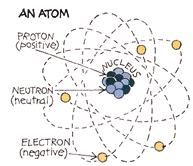
\includegraphics[width=1.0in]{atom.jpg},\centerline{The Atom}] The \verb+multicols+ package allows using multiple columns without starting a new page.  Using floats is not possible in a columns environment, however with the \verb+picinpar+ package, I can set a picture inside a block of text---just like you one you see here.  Isn't \LaTeX{} cool?
And now we're just filling more space, and yet more space.  
\end{window}
\closearticle


\headline{\it\huge Another Headline}
This is just an example to fill up some space, but as long as I have your attention, I'll give some newspaper advice.

It's good to use different fonts for each headline.  This particular font was accomplished with the command \verb+\headline{\it\huge Another Headline}+.  The headline in the preceding article was accomplished with the command \verb+\byline{\sc\Large Geek Designs New \LaTeX{} Package}{Matthew Allen}+.

Of course the commands don't look so nice when they're set in column format.  Look at the example file if you have any questions as to how this example was created.

I suppose we could also show how an equation is type set:
\begin{displaymath}
x=\frac{-b\pm\sqrt{b^2-4ac}}{2a}
\end{displaymath}
and there you have it.  \closearticle
}
\end{multicols}

\end{document}